\section{Teilversuch 6: Fresnel Beugung an der Kante}
	Aus der Anleitung soll die Transmission so aussehen:
	\begin{figure}[H]
		\centering
		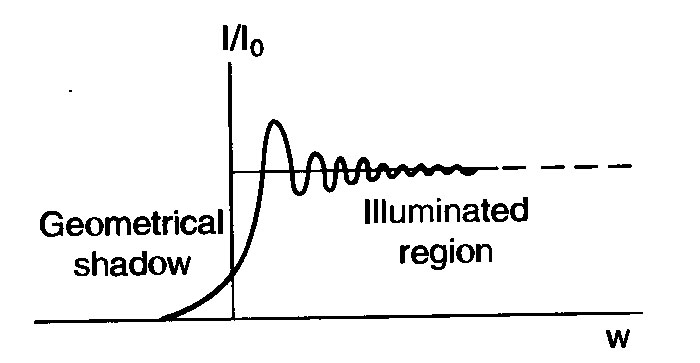
\includegraphics[width=0.5\textwidth]{images/kante.jpg}
		\caption{\textcolor{gray}{Abbildung aus Anleitung BEU Seite 14 §1.9 Abbildung 10 rechts}}
		\label{fig:kante-trans}
	\end{figure}
	Also zeigt die Intensität auf der Lichtseite Maxima und Minima. Die Amplitude dieser Oszillation soll auch mit zunehmender Entfernung vom Schatten abnehmen. 

	Das ist genau was wir im Experiment beobachtet haben. Ein Unterschied ist aber, dass die Transmission mit zunehmender Pixelzahl zunimmt. Das liegt vermutlich daran, dass den Laserstrahl eine endliche Durchmesser hat. 